%%%
%
% $Autor: Deepti Hegde $
% $Datum: 2023-02-26 $

%
% !TeX spellcheck = de_DE/GB
%
%%%



\chapter{Technical Specifications of Arduino Nano 33 BLE Sense}


\fcolorbox{yellow}{yellow!10}{\begin{minipage}{\textwidth}
		\begin{center}
			\begin{tabular}{llm{90mm}} 
				%\multicolumn{3}{l}{\large \textcolor{blue}{ Tech Specs of Arduino Nano 33 BLE Sense}} \\ \hline
				\\ \textbf{\MapleCommand{MICROCONTROLLER}}  & nRF52840\\
				\textbf{\MapleCommand{OPERATING VOLTAGE}}  & 3.3V\\
				\textbf{\MapleCommand{INPUT VOLTAGE (LIMIT)}}  & 21V \\
				\textbf{\MapleCommand{DC CURRENT PER I/O PIN}}  & 15 mA \\
				\textbf{\MapleCommand{CLOCK SPEED}} & 64MHz \\
				\textbf{\MapleCommand{CPU FLASH MEMORY}}  & 1MB  \\
				\textbf{\MapleCommand{SRAM}}  & 256KB  \\
				\textbf{\MapleCommand{EEPROM}}  & None  \\
				\textbf{\MapleCommand{Digital Input/Output Pins}}  & 14  \\
				\textbf{\MapleCommand{PWM Pins}}  & all digital pins  \\
				\textbf{\MapleCommand{UART}}  & 1 \\
				\textbf{\MapleCommand{SPI}}  & 1 \\
				\textbf{\MapleCommand{I2C}}  & 1 \\
				\textbf{\MapleCommand{Analog Input Pins}}  & 8(ADC 12 bit 200 k samples) \\
				\textbf{\MapleCommand{Analog Output Pins}}  & Only through PWN (no DAC) \\
				\textbf{\MapleCommand{External Interrupts}}  & all digital pins \\
				\textbf{\MapleCommand{LED\_BUILTIN}}  & 13 \\
				\textbf{\MapleCommand{USB}}  & Native in the nRF52840 Processor \\
				\textbf{\MapleCommand{IMU(Accelerometer, Gyroscope, Magnetometer)}}  & LSM9DS1 \\
				\textbf{\MapleCommand{MICROPHONE}}  & MP34DT05 \\
				\textbf{\MapleCommand {Gesture, Light, Proximity Sensor}}  & APDS9960 \\
				\textbf{\MapleCommand{Barometric Pressure Sensor}}  & LPS22HB \\
				\textbf{\MapleCommand{Temperature, HumiditySensor}}  & HTS221 \\
				\textbf{\MapleCommand{Dimensions Width x Length}}  & 18 x 45 mm \\
				\textbf{\MapleCommand{Weight}}  & 5 g (with headers) \\
			\end{tabular}
			\captionof{table}{Technical Specifications of Arduino Nano 33 BLE Sense \cite{Ard:2019}}
		\end{center}
\end{minipage}}

\begin{figure}[h!]
	\centering	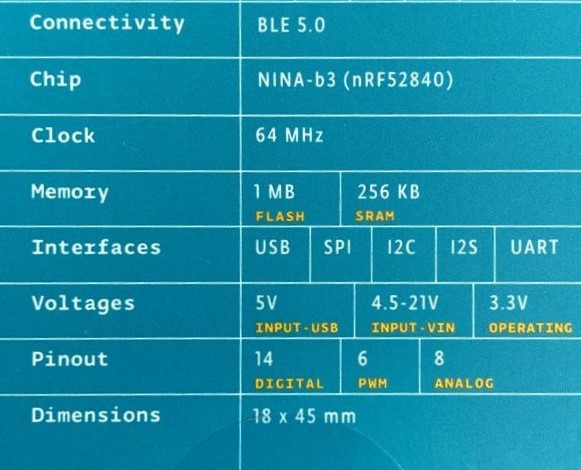
\includegraphics[width=9cm]{Images/spec}
	\caption{\textbf{Technical Specification}}
\end{figure}
